%==============================================================================
% document template for a LaTeX file
% Created : 22.11.2006 by Romain de Wolff
% Modif : 8 octobre 2007, respect standart HEIG-VD pour travaux de diplômes
%==============================================================================
% configurations du document
\documentclass[a4paper, 11pt]{article}
\usepackage[utf8]{inputenc}
\usepackage[cyr]{aeguill}
\usepackage[frenchb]{babel}               % \og et \fg pour les guillemets
\usepackage{url}                          % pour inclure des URLs
\usepackage{color}                        % utilisé pour le code source
\usepackage{listings}                     % pour inclure le code source
\usepackage{geometry}                     % pour les marges
\usepackage{algorithmic}                  % pour présenter les algos
\usepackage{algorithm}                    % pour présenter les algos
\usepackage{graphicx}                     % pour inclure des images
\usepackage{fancyvrb}                     % pour avoir du verbatim encadré
\usepackage{url}                          % pour inclure des URLs
\usepackage{geometry}                     % See geometry.pdf to learn the layout options
\usepackage{moreverb}					  % permet d'encadrer le verbatim à l'aide de la commande \begin{boxedverbatim}
\usepackage{longtable}

\geometry{a4paper}                        % ... or a4paper or a5paper or ... 
%\geometry{landscape}                     % Activate for for rotated page geometry
\usepackage[parfill]{parskip}             % Activate to begin paragraphs with an empty line rather than an indent
%\usepackage{amssymb}
%\usepackage{epstopdf}                    % Pour créer des références divers (webographie, etc) 
\usepackage{bibtopic}
\geometry{ hmargin=2.8cm, vmargin=2.5cm } % marges
%==============================================================================
% debut macro 
% permet de mettre en gros la premiere lettre d'un paragraphe
\font\capfont=cmbx12 at 44.87 pt % or yinit, or...?
\newbox\capbox \newcount\capl \def\a{A}
\def\docappar{\medbreak\noindent\setbox\capbox\hbox{%
\capfont\a\hskip0.15em}\hangindent=\wd\capbox%
\capl=\ht\capbox\divide\capl by\baselineskip\advance\capl by1%
\hangafter=-\capl%
\hbox{\vbox to8pt{\hbox to0pt{\hss\box\capbox}\vss}}}
\def\cappar{\afterassignment\docappar\noexpand\let\a }
% fin macro
%==============================================================================

%==============================================================================
% première page
\title{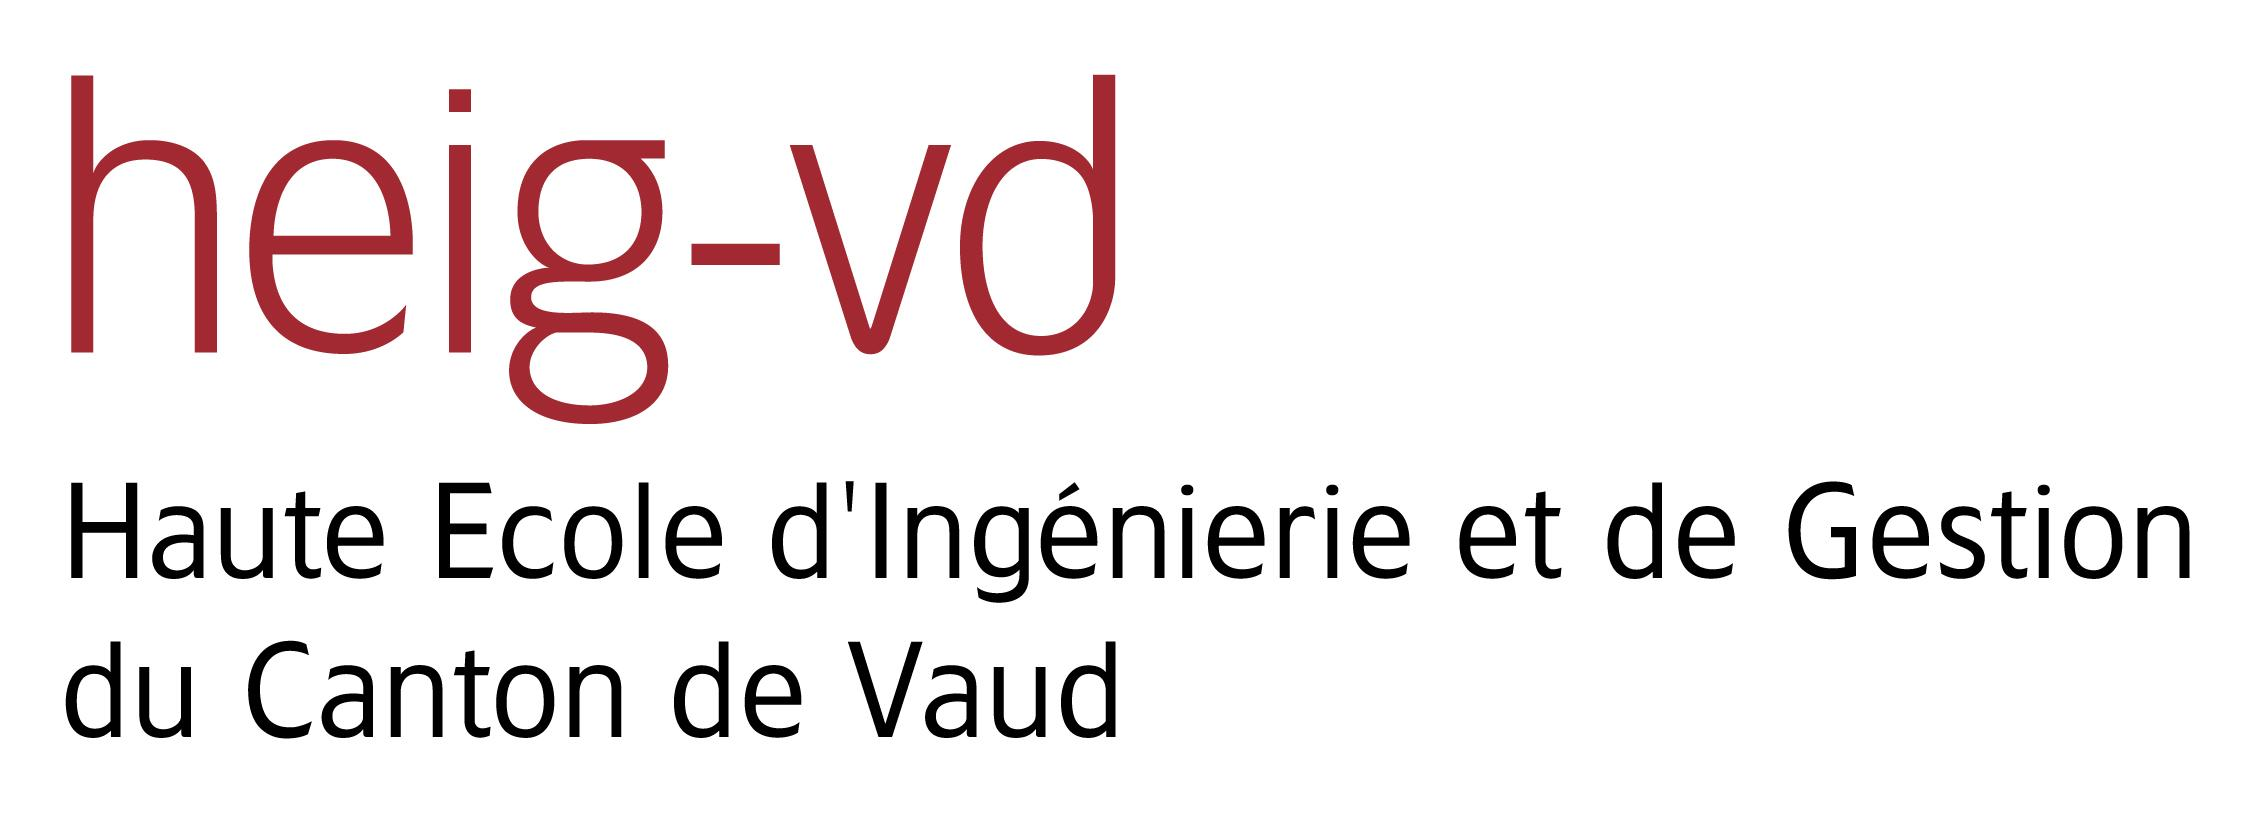
\includegraphics[width=100px]{HEIG-VD.jpg} \\ \vspace{4cm}
\small{PPE - Présentation personnelle} \\ \vspace{2cm}
\huge{WebDAV} \\ \vspace{1cm} 
Web-based Distributed Authoring and Versioning \\ 
\small{Un protocole réseau pour l'édition collaborative sur le web}} 
\vspace{2cm}
\author{Romain \bsc{de
Wolff} \\ IL2008 \\ \vspace{2cm} \\ Professeurs Mme. Laura Elena Raileanu \\ et Mme Nastaran Fatemi \vspace{2cm} 
}
\date{Lausanne, le 8 octobre 2007}  % Activate to display a given date or no date
\pagebreak{}
\begin{document}
\maketitle
\thispagestyle{empty} % enlève le numéro de page sur la page de titre (uniquement)
\newpage
%==============================================================================
% configuration des numérotations de pages (chiffres romains)
\pagenumbering{roman} \setcounter{page}{1} 

% Configuration de la distance d'interligne 
{\setlength{\baselineskip}{1.2\baselineskip}
% Configureation de la distance entre les paragraphes
\parskip=12pt
%==============================================================================

%==============================================================================
\section*{Remerciements} 
%==============================================================================

@end

%==============================================================================
\section*{Résumé}
%==============================================================================

@end

% protocole réseau, créer un sorte de système de fichier partageable, network drive,
% collaboration, vesrsion, sauvegarde, sécurité, etc.. :)
% notion informatique REQUISES... UTF8, UTF16, système de ficheir, etc... 

% TODO : prérequis ? base de HTTP, mais survolé. XML etc... 

%==============================================================================
% Table des matières
\newpage
\tableofcontents
\newpage
%==============================================================================
% reconfiguration des numéro de pages (on recommence a compter a 1)
\pagenumbering{arabic} \setcounter{page}{1} 
%==============================================================================

%==============================================================================
\section{Introduction}
%==============================================================================

	% décrire le problème, l'objectif et la motivation
	% attirer le lecteur
	% http://www.asis.org/Bulletin/Oct-98/webdav.html-> printé

	% problème - comment ca marchait dans le passé? - exemple - temps, etc..

	\cappar Internet met aujourd'hui à disposition de tout le monde une quantité d'informations qui ne cesse de croître. Ces dernières années, la quantité d'informations disponible a carrément explosé. N'importe quel ordinateur connecté à internet peut accéder à ce vaste réseau et à toute ces données. L'utilisateur peut naviguer de page en page et aux travers de gros index d'une manière très simple et efficace. De se fait il peut consulter des textes, des images, des vidéos sans fin. Ou presque. 
	
	Cette interopérabilité fut possible grâce a deux standards aujourd'hui : \emph{HyperText Markup Language} (HTML) et \emph{HyperText Transfer Protocol} (HTTP). Ces deux standards sont disponible sur tout type d'ordinateur, allant même, aujourd'hui, jusqu'au téléphone portable. Ainsi le nouveau téléphone d'Apple, le \emph{iPhone}, implémente \emph{Safari}, qui respectent les standards HTML actuels. Quelqu'un désireux de créer un site internet peut le faire à l'aide d'un ordinateur bon marché ainsi que d'une connexion internet. Une fois son document déposé sur le web, n'importe qui peut y accéder et y faire référence. C'est ce qui rend le \emph{World Wide Web} plus ouvert que n'importe quel système connu à ce jour. 
	
	Quand Tim Berners-Lee écrit la première page HTML au CERN\footnote{Organisation Européenne pour la Recherche Nucléaire. A l'origine, c'était l'acronyme du Conseil Européen pour la Recherche Nucléaire. \url{http://www.cern.ch}. Un organe provisoire institué en 1952, qui avait pour mandat de créer en Europe une organisation de rang mondial pour la recherche en physique fondamentale} c'était dans le but de mettre des textes scientifique en ligne et de pouvoir se référer entre eux sans créer une base de données centralisée. % + collaboratifs 
	
	Quand le web apparu auprès du public, la plupart des clients pouvaient parcourir l'information mais pas l'éditer. Lire des informations était le plus important et le plus facile. Editer est plus complexe. L'engouement du début se concentra sur la lecture et en oublia l'écriture. Quelques protocoles propriétaires émergèrent rapidement, mais durant près de 10 ans, aucun standard d'écriture sur le web n'était disponible. 
	
	\subsection{Qu'est ce que WebDAV?}
	
	\emph{Web-based Distributed Authoring and Versioning} (WebDAV), est le premier protocole standard d'écriture sur le web. En Anglais, on utilise le mot \emph{authoring}, qui défini bien ce qu'offre WebDAV, aussi souvent appelé simplement \emph{DAV}. Cela signifie auteur, écrivain, créateur. WebDAV met en place une série de fonctionnalité qui permet de créer des documents sur internet en collaboration. La RFC 2518\footnote{La RFC 2518 est disponible en français à l'adresse \url{http://www.webdav.org/specs/rfc2518.fr.html}} décrit les spécifications que défini ce nouveau protocole. Le but de WebDAV est de mettre à disposition l'écriture de la même manière que la lecture. Il est construit sur le protocole HTTP et y ajoute des fonctionnalités d'écriture et de gestions des documents. Il permet aussi de gérer l'évolution des modifications (\emph{versioning}) ainsi que le l'écriture d'un même document par plusieurs auteurs.
		
		WebDAV nous permet donc d'éditer \emph{directement sur le serveur HTTP}, ce qui nous permet de ne pas utiliser simplement le web comme media de lecture, mais aussi comme média d'écriture collaboratif. 
		
		
		% TODO: objectif de WebDAV : répondu ?
		
		% ajouter : p 37 livre : top : partage de _tout_ type de documents !!

%==============================================================================
\section{Un peu d'histoire}
%==============================================================================

	% TODO : référence au livre dont j'utilise les passages pour reprendre l'histoire
	
	Quand Tim Berners-Lee et Robert Cailliau inventère le \emph{World Wide Web}, ils voulaient rendre l'édition de fichiers aussi facile que la lecture d'un document. C'est pour cela que HTTP inclus deux méthodes qui permettent en théorie de mettre à jour les pages web : \emph{PUT} pour créer ou modifier un fichier, et \emph{DELETE} pour effacer. Mais rapidement les utilisateurs ont utilisés le transfert de fichier sur internet (FTP, \emph{File Transfer Protocol}). Le HTTP ne fonctionnait pas pour eux pour plusieurs raisons : 

	\begin{itemize}
		\item 	La sécurité n'était pas bonne. A cause de cela beaucoup d'administrateurs désactivèrent \emph{PUT} et \emph{DELETE}.
		\item 	HTTP n'a pas de concept de collections, ce qui rendait impossible la création d'une page a un endroit spécifique voulu
		\item 	Les premiers navigateurs se concentrèrent sur la lecture de document et ne supportaient pas l'écriture. Les éditeurs de textes ne supportaient pas le HTTP. C'est pour cela qu'il fallait utiliser un autre outil pour modifier sa page et un autre pour l'envoyer sur le serveur HTTP.
	\end{itemize}
			
	\subsection{Au tout début}
	
		Les premiers sites internet furent forcément créés à l'aide d'éditeur de texte conventionnel car il n'existait pas encore d'outils spécialisés. Si l'auteur ne se trouvait pas directement sur la serveur HTTP, il utilisait souvent le protocole FTP (\emph{File Transfer Protocol}) pour mettre ces fichiers HTML terminé sur le serveur web. 

		Le protocole FTP était un standard depuis 1985, bien avant que HTTP ne naisse. Il n'a donc pas été créé pour éditer des pages HTML. Il ne gère pas non plus le fait que plusieurs personnes éditent le même fichier en même temps. 

		Les premiers outils utilisés pour remédier a ce manque furent les éditeurs HTML. Ils mirent à disposition des fonctionnalités plus ou moins avancées pour travailler sur des fichiers HTML. En local, cela fonctionnait très bien, mais dès qu'il fallait travailler sur des serveur à distance, le problème n'était pas vraiment résolu.

	\subsection{Logiciels propriétaires}
	
		Pour remédier aux problèmes de création et de mise à jour de fichiers sur un serveur web, les entreprises de création de logiciels ont crée des programmes propriétaires qui permettaient de faire cela. Mais chacun avec ses propres méthodes. Les outils étaient donc très souvent incompatible les uns des autres. 
		
		\begin{itemize}
			\item \emph{Vermeer FrontPage} qui devint \emph{Microsoft FrontPage}, utilisa un protocole propriétaire pour gérer les fichiers à distances	
			\item 		\emph{Macromedia Dreamweaver} et \emph{Allaire Coldfusion} eurent la capacité d'écrire des pages de manière collaboratives, avec la possibilité de verrouiller un fichier afin qu'un seul auteur le modifie à la fois. Mais cela fonctionnait au travers de protocoles propriétaires uniquement
			\item 		\emph{Nestcape Navigator Gold} avait la capacité d'envoyer des fichiers sur un serveur distant en utilisant \emph{FTP} ou \emph{HTTP PUT}. Cela fonctionnait bien si un seul auteur utilisait le serveur, mais pas pour plusieurs.
		\end{itemize}
		
		Les équipes de développement web professionnelles utilisent de temps en temps des systèmes de gestion des sources appelé \emph{CM} (Configuration Management). \emph{CVS} ou \emph{Subversion} sous Unix et \emph{Microsoft SourceSafe} sont tout deux des serveurs \emph{CM}. Ces systèmes utilisent souvent des protocoles personnalisés qui rendent difficile le support d'autres applications. Malgré le fait qu'ils offrent d'excellentes fonctionnalités pour la gestions d'utilisateurs multiples et la gestion des versions, ils forcent les développeurs à recopier les fichiers sur le serveur en production. Car il n'est pas pratique et souvent pas désirable de modifier les pages web directement sur un environnement de production.
	
	\subsection{Edition au travers des formulaires web}
	
		Beaucoup de fournisseur d'accès internet ou d'autres grand site internet de services comme \emph{Yahoo} offrent la possibilité d'héberger un site internet de petite taille gratuitement. Ils hébergent donc des sites pour un grand nombre de personnes. 
		
		Ces services utilisent les formulaires HTML pour la création et la modification de leur pages. Les utilisateurs peuvent entrer des information dans des champs de textes que le serveur mettra en ligne pour eux de manière automatique. Naturellement, les fonctionnalités sont ici très simples et l'utilisateur n'a pas beaucoup de possibilités. 
		
		Ce système permet aux utilisateurs de n'avoir aucun logiciel particulier pour mettre en forme leur pages. Ils utilisent directement leur navigateur web pour ce faire. 
		
		Aujourd'hui ce système c'est très développé avec l'apparition récente des BLOG\footnote{Raccourcis de \emph{Web Log}. C'est une sorte de journal privé dont le contenu est souvent textuel} qui permet de créer des facilement articles aux travers d'une interface web.
		
		Tout ces mécanismes souffrent malheureusement d'un gros défaut : ils ont pour but d'être édité par un seul et unique auteur. 

	% download http - upload ftp - email exchange document	
	\subsection{Le travail collaboratif avant WebDAV}

		Pendant des années, le travail en collaboration s'effectuait comme cela : télécharger le document via HTTP, échanger les fichiers avec d'autres auteurs par e-mails et envoyer les documents sur le serveur par FTP. C'était un peu \emph{l'âge de pierre} de l'édition web. Avant qu'aucun outil ou nouveau protocole n'existe. Les seuls logiciels qui existaient était des clients (navigateurs) et serveurs HTTP. Ceux-ci étaient tout d'abord uniquement disponible dans le monde \emph{Unix}, mais se développèrent aussi vite dans le monde \emph{Windows}.
		
		Entre 1995 et 1998 l'accroissement de l'utilisation d'internet fut le déclencheur denouveaux départs. L'arrivée de \emph{Microsoft Windows 95} fit grandement évoluer les choses. En effet, les clients Unix furent de moins en moins seuls sur le marché et cela contribua fortement aux développement du web. Les clients Mac suivirent très peu après. Le grand engouement pour cette technologie fit vite part à un manque . En effet il était difficile d'utiliser Telnet, FTP ou NFS pour des utilisateurs habitués à une interface graphique. 
		
	Dès lors, les programmes propriétaires tentèrent d'implémenter des extensions serveurs qui permettaient de combler ces lacunes. Mais chaque client communiquait uniquement avec son serveur correspondant. Aucun standard n'était présent sur le marché. Chacun utilisait son propre protocole sans vraiment tenir compte de celui des autres. Ou alors un standard ouvert mais pas suffisamment complet pour une utilisation à grande échelle était utilisé.
		
	% troisieme generation
	\subsection{La formation de WebDAV}
	
		Les équipes partagent les mêmes ressources web devinrent de plus en plus grandes. L'accroissement économique du Web acquérit une telle importance que ce n'était plus un ou deux experts qui géraient un site web, mais toute une équipe d'une grande organisation.
		
		Les outils étaient trop diversifiés pour que le travail se fasse de manière simple. Chacun modifiait ses fichiers de son côté et les plaçaient sur le serveur une fois le travail terminé. Il n'était pas rare que des données soit perdues.
		
		Finalement, en 1996, les vendeurs de plusieurs de ces programmes informatiques réussirent à se regrouper et décidèrent de faire l'effort de créer un standard ensemble. Leurs désirs étaient de créer un protocole permettant d'utiliser n'importe quel outil Web ou de bureautique afin de modifier un fichier à distance sur une serveur web. Pour rendre ceci possible, il fallait créer un nouveau protocole commun.
		
		C'est comme ça que naquit WebDAV! Il créèrent un nouveau protocole, car il n'était pas envisageable de choisir le protocole déjà établis par une entreprise. En effet, cela aurait avantagé la société de manière considérable.

		Après des années de travail et de discussion, IETF, l'Internet Engineering Task Force, définit WebDAV comme un standard. C'est en 1998 que fût proposé la version finale du protocole WebDAV. Il fût accepté en 1999 et devint un standard, dont nous connaissons aujourd'hui la RFC 2518.
		
%==============================================================================
\section{Spécifications}
%==============================================================================

	C'est l'IETF qui maintient à jour les spécifications de WebDAV. L'IETF (\url{http://www.ietf.org}) est une large communauté internationale de réseaux de designer, opérateur, vendeurs et scientifiques concernés par l'évolution d'internet. Ils sont particulièrement concernés par l'architecture et le bon fonctionnement des opérations sur internet. La communauté est ouverte a tout le monde qui s'intéresse de près ou de loin à ce sujet. Les buts de l'IETF sont regroupé dans la RFC 3935.	
	
	\subsection{Problèmes à résoudre}
	
		% TODO
	
	\subsection{Solution proposées}
	
		% TODO
	
	\subsection{Architecture client-serveur}	
	
		% TODO
	
%==============================================================================
\section{Mécanismes HTTP}
%==============================================================================

WebDAV est basé sur le protocole HTTP. Il utilise les mêmes requêtes, réponses, méthodes et code d'erreurs. Beaucoup d'en-tête de HTTP sont réutilisées dans WebDAV et d'autres sont rajoutées. Les requêtes et les réponses de WebDAV passent à travers les proxy et les pare-feux. C'est un des avantages de l'utilisation d'un protocole aussi répandu que HTTP.

WebDAV a de nombreuses fonctionnalités basée sur le protocole HTTP, et qui sont aussi uniquement documentée dans ces spécifications, il est donc important de passer en revue quelques points important de ce protocole. 

Ce chapitre est un survol des possibilités offertes par le protocole HTTP, tout en mettant un accent sur les fonctionnalité ayant une corrélation plus forte avec le protocole WebDAV.

Une section de chapitre (cf. section \ref{sub:modif_proto_http}, page \pageref{sub:modif_proto_http}) est consacrée aux modifications apportées au protocole HTTP décrit ci-dessous.

	\subsection{URL et URI}
	
		Les \emph{Uniform Resource Locator} (URL) est une adresse vers une ressource digitale. Leur ordre et leur structure est définie de manière stricte.
		
		Par exemple : \url{http://www.exemple.com:8080/path/index.html} 
		
		\begin{itemize}
			\item \verb$http://$ représente le protocole utilisé. Le client qui reconnaît ce protocole pourra déterminer la structure de la suite de l'adresse. Un autre protocole peut avoir une structure différente.
			\item \verb$www.exemple.com$ l'adresse du serveur. Cette adresse est liée a une adresse IP qui est déterminée a l'aide des serveur de noms (DNS, Domain Name Server, dont le protocole est le défini dans la RFC 1035)
			\item \verb$8080$ le port sur lequel la connexion TCP sera établie
			\item \verb$/path/index.html$ indique le chemin qui sera demandé au serveur
		\end{itemize}
		
		On utilise la nomenclature \emph{Uniform Resource Identifier} (URI) de manière plus générale. Une URL est une URI. Une URI défini de manière général comment atteindre une ressource, un nom ou les deux. Sa syntaxe globale est définie de manière précise, puis, chaque protocole défini sa propre hiérarchie. On peut citer des exemples tel que \texttt{HTTP}, \texttt{FTP}, \texttt{mailto}, \texttt{URN}, \texttt{rtsp}, etc...
		
	\subsection{Requêtes HTTP}
	
		Une requêtes HTTP doit comporter une méthode, une URL et la version du protocole utilisée. Elle peut contenir des en-têtes (chacune dans une ligne séparée), ainsi qu'un corps (body) optionnel. La figure \ref{fig:req_http} montre un exemple de requête HTTP envoyé à un serveur.
		
		\begin{figure}[ht]
		\begin{center}
		\begin{boxedverbatim}
			GET /index.html HTTP/1.1
			Host: exemple.com:8080
			Content-Length: 1200
			
			Le corps doit contenir le nombre de caractères spécifié dans l'en-tête
		\end{boxedverbatim}
		\caption{Un exemple de requête HTTP envoyé au serveur}
		\label{fig:req_http}
		\end{center}
		\end{figure}
		
		\texttt{GET} spécifie la méthode utilisée. \texttt{/index.html} est l'URL relative et \texttt{HTTP/1.1} le protocole et sa version. Les deux lignes suivantes définissent les en-têtes. Après la ligne blanche qui est requise se trouve éventuellement le corps. 
		
	\subsection{Réponses HTTP}
	
		Les réponses HTTP ont une structure légèrement différentes. Elles comportent tout d'abord une ligne de statut, les en-têtes, une ligne vide puis les corps, toujours optionnel. 
		
		La ligne de statut comporte dans l'ordre, le protocole utilisé ainsi que sa version, le code de statut et une description du statut. La figure \ref{fig:rep_http} montre un exemple de réponse HTTP.
		
		\begin{figure}[ht]
		\begin{center}	
		\begin{boxedverbatim}
			HTTP/1.1 200 OK
			Date: Sun, 19 Sept 2007 23:30:12 GMT
			Content-Length: 1200
						
			Le corps doit contenir le nombre de caractères spécifié dans l'en-tête
		\end{boxedverbatim}
		\caption{Un exemple de réponse HTTP retourné par le serveur}
		\label{fig:rep_http}
		\end{center}
		\end{figure}

	\subsection{Méthodes HTTP}
		
		\textsc{GET} est une méthode définie par le protocole \texttt{HTTP}. Il en existe d'autres, commme  \texttt{PUT}, \texttt{DELETE}, \texttt{POST}, \texttt{HEAD} et \texttt{OPTIONS}. Elles sont toutes des méthodes utiles pour l'édition collaborative. Voici une liste non exhaustive de ces méthodes et de leurs fonctions : 
		
		\begin{itemize}
			\item GET : récupère un document spécifique 
			\item PUT : ajouter ou modifie un document
			\item DELETE : efface une ressource 
			\item POST : utilisé dans les formulaires web, il permet d'envoyer un fichier sur le serveur
			\item HEAD : retourne les mêmes informations qu'un \texttt{GET}, mais sans le corps
			\item OPTIONS : demande les méthodes supportée sur un élément précis
		\end{itemize}
		
		Le chapitre \ref{sec:proto_webdav} décrit plus en détail le protocole WebDAV. 
		
%==============================================================================
\section{Le protocole WebDAV}
\label{sec:proto_webdav}
%==============================================================================

%TODO : sujet : petite introduction. pas de -V- au début

Le protocole \texttt{HTTP/1.1} est conçu de manière simple : tout les objets web sont des ressources que l'on identifie par une \texttt{URI}. WebDAV étends cette structure, tout en la gardant simple.

\begin{itemize}
	\item La notion de collections est ajoutée. C'est une structure particulière qui permet de contenir d'autres ressources. 
	\item Toute les ressources ont des propriétés (nom, valeur). Les propriétés ne sont pas directement adressables et n'ont pas d'\texttt{URI}.
	\item Chaque ressource peut être verrouillée . C'est une concept fondamentale afin de pouvoir gérer le travail collaboratif correctement. On parle de \texttt{locks}, \emph{serrure} en anglais.
\end{itemize}


Nous allons voir plus en détail ces éléments ainsi que d'autres, afin de mieux comprendre l'interaction dans le protocole WebDAV. 

	\subsection{Structure et ressources}
	
		Une \textbf{ressource WebDAV} est un objet web que l'on identifie par une adresse, comme par exemple un fichier ou un répertoire. Il peut contenir n'importe quel type \texttt{MIME} (RFC 2045). Cela implique du \texttt{HTML}, du texte normal, des images ou n'importe quel document d'une suite bureautique. De plus, cet élément contient un verrou ainsi que des propriétés. 
		
		WebDAV reprend ainsi exactement ces ressources comme défini dans le protocole HTTP. C'est très utile, car avec la même adresse on peut accéder a un fichier, et avec WebDAV, on peut s'identifier (il faut bien sûr penser à la sécurité) afin de modifier ce même contenu.
		
		Les ressources sont structurées comme un système de fichiers en arborescence. La figure \ref{fig:file_structure} illustre la hiérarchie d'une partie de site internet. 

		\begin{figure}[htc]
		\begin{center}
		\includegraphics[width=204px]{schemas/URL-Hierarchie.png}
		\caption{Une hiérarchie basée sur la structure des URLs}
		\label{fig:file_structure}
		\end{center}
		\end{figure}
		
		On parle plutôt de \emph{ressource} que de fichier ou de dossier. La terminologie ressource est bien définie et permet d'identifier les deux objets à l'aide d'un seul mot. Le terme \textbf{collection} fait toujours référence à une collection d'objet WebDAV. Un fichier ou un dossier est un élément propre à un système de fichier hors du contexte de WebDAV. On parle aussi de \textbf{parent} et d'\textbf{enfant}

	\subsection{Propriétés}
	
		Le web regorge d'informations. Retrouver un fichier uniquement par son nom n'est pas une solution viable à cette échelle. Les propriétés, dans WebDAV on parle de \textbf{Metadata}, permettent d'ajouter des informations à propos d'une ressource. C'est un système fondamental ainsi que d'une utilité cruciale. 
		
		Ces propriétés possède un autre atout : il n'est pas nécessaire de télécharger un document en entier afin d'en soutirer les informations. Ainsi une image qui contient son copyright dans un champs du fichier (\textbf{JPEG} par exemple), implique un téléchargement complet de l'image. Le téléchargement est nécessaire afin de trouver uniquement une petite information. Les propriétés permettent d'éviter ce problème. WebDAV permet de stocker les propriétés hors du corps d'un fichier.
		
		Les méthodes \texttt{PROPFIND} et \texttt{PROPPATCH} permettent respectivement de chercher ou de modifier les propriétés d'un fichier. Les propriétés sont des paires de valeurs toujours stockées en chaîne de caractères Unicode. Typiquement en UTF-8 ou UTF-16. Le client et le serveur peuvent négocier d'autre encodage de caractères. N'importe quelle objet structuré peut être transformé en chaîne de caractère et donc y être stocké. La gestion des propriétés est un système puissant que fournit WebDAV.
		
		Les deux méthodes \texttt{PROPFIND} et \texttt{PROPPATCH} utilisent le XML pour gérer et structurer les propriétés\footnote{L'IETF est un groupe formé par le W3C, qui est le père du XML}. Des propriétés ne contenant aucune valeur sont tout à fait possible. Une requête pour une propriété non existante va retourner un code d'erreur 404, alors que la même requête sur une propriété vide retournera un champs vide. 
		
		Il existe plusieurs différents types de propriétés. Les propriétés dite \textbf{live}, et a l'opposé les propriétés dite \textbf{dead}. Par définition, une propriété \textbf{live} inclus : 
		
		\begin{itemize}
			\item Les propriétés calculées par le serveur, comme la date et l'heure
			\item Les propriétés protégées, que le client ne peut pas modifier
			\item Les propriétés utilisées comme informations de configuration
			\item Les propriétés dont le serveur vérifie la syntaxe ou le type de données
		\end{itemize}
		
		Les autres dites \textbf{dead} ou mortes en français, sont celles qui sont écrites et lues par les clients sans interférences de la part du serveur WebDAV. Un exemple de ce type de propriété est le \emph{Nom complet}. Le serveur n'en vérifie pas le contenu.
		
		% TODO éventuellement  : move and copy and properties : pp 94-95
		
		Les propriétés sont donc des éléments XML. Des règles strictes les définissent. Chaque propriété se doit d'être unique, dans le but d'éviter toute confusion sur le serveur. Cela permet de garantir une interopérabilité maximum. De plus, elles sont sensible à la casse.
		
		Le tableau \ref{tab:ex_prop} montre quelques exemples de propriétés.
		
		\begin{table}[htc]
		\begin{center}
			\begin{tabular}{p{4cm}|p{4cm}|p{3.5cm}|p{2cm}}
			\hline
			\hline
			Propriété & Signification & Disponible dans & Protégé \\
			\hline
			creationdate & La date et l'heure à laquelle la ressource a été crée & Toute les ressources & Oui \\
			\hline
			displayname & le nom de la ressource a afficher aux utilisateurs & Tout les ressources & Peut l'être \\
			\hline
			getcontentlanguage & la taille de la ressource & Tout les ressources qui répondent à un GET & Oui \\
			\hline
			lockdiscovery & détail sur les information du ou des éventuels verrous & Toute les ressources verrouillées & Oui \\
			\hline
			\end{tabular}
		\caption{Une hiérarchie basée sur la structure des URLs}
		\label{tab:ex_prop}
		\end{center}
		\end{table}
		
		La valeur des propriétés est donc du XML. Une propriété se caractérise donc par un nom situé entre < et >. Un exemple est montré dans la figure \ref{fig:ex_prop}. 
		
		\begin{figure}[ht]
		\begin{center}	
		\begin{boxedverbatim}
			<nomDeLaPropriete>
				Valeur
			</nomDeLaPropriete>
		\end{boxedverbatim}
		\caption{Un exemple de propriété en XML ainsi que de sa valeur}
		\label{fig:ex_prop}
		\end{center}
		\end{figure}

		% TODO if time : chapitre 7, p 145 : opérations sur les propriétés

	\subsection{Verrouillage}
	
		Les verrous en WebDAV existent afin d'éviter que des utilisateur n'écrasent le travail des autres accidentellement. Le verrouillage est une fonctionnalité optionnel de WebDAV. Il est donc possible de désactiver. Mais un client qui se connecte a un server WebDAV se doit d'être prêt a recevoir une erreur si il tente de modifier un fichier verrouillé.
		
		WebDAV met à disposition uniquement des \textbf{verrous d'écriture}. Ceci protège contre toute opération d'écriture comme le \texttt{PUT}, \texttt{PROPPATCH}, \texttt{MOVE} ou encore \texttt{COPY}. Par contre le faite de verrouiller un document n'empêche pas la lecture des information qu'il contient. Pendant qu'un fichier est verrouillé, les utilisateur ne possédant pas le verrou peuvent toujours télécharger le fichier. 
		
		Les verrous possèdent une durée de vie définie, qui peut être limitée ou infinie. La possibilité de définir un temps d'expiration d'un verrou est très utile. En effet, on peut imaginer qu'un client oublie qu'il a la main sur un fichier, ou qu'il crash tout simplement. Il existe la notion de rafraîchissement des verrous. Ceci afin d'être certain que tant qu'un client modifie un fichier, il garde le verrou. Par exemple un logiciel peut détecter que le client est entrain d'effectuer des modifications sur le fichier et de se fait, envoyer des requêtes au serveur WebDAV afin de maintenir le verrou actif. 
		
		Tous les verrous possèdent aussi un identifiant unique qui est utilisé pour toute opérations les concernants qu'on effectue. 
	
			\begin{figure}[htc]
			\begin{center}
			\includegraphics[width=400px]{schemas/Ressource-Locks.png}
			\caption{Des ressources ainsi que leurs propriétés et un verrou sur un objet}
			\label{fig:file_lock}
			\end{center}
			\end{figure}
		
		Tous les verrous possède un propriétaire. Ceci afin d'éviter qu'une autre personne puisse modifier le fichier durant ce temps. Les identifiants des verrous sont publique. Et cela pourrait être un problème. En effet n'importe qui pourrait trouver le numéro d'un verrou et le déverrouiller. Heureusement ce n'est pas possible car uniquement l'utilisateur qui possède le verrou peut le modifier.
		
		\begin{itemize}
			\item Quand un verrou est crée, le serveur doit stocker l'identité de l'utilisateur qui l'a crée
			\item Quand une mise à jour sur le fichier (ou un rafraîchissement du verrou ou un déverrouillage) est effectuée, le serveur doit vérifier le numéro de verrou ainsi que l'identité de l'utilisateur
			\item Si l'identité de l'utilisateur ou le numéro du verrou est manquant, le serveur doit retourner une erreur. Il existe un cas quand le serveur est publiquement modifiable ou il est éventuellement possible de ne pas connaître l'identité de l'utilisateur
		\end{itemize}
		
		Le verrouillage des ressources mise à disposition par WebDAV résous le problème de la mise à jour perdue lorsque deux ou plusieurs utilisateurs veulent modifier une ressource. Grâce au fait que le ressource soit bloquée durant son édition, personne d'autre ne peut modifier le même fichier. Une fois que le fichier est déverrouillé, un autre utilisateur pourra reprendre le contenu de ce fichier et le mettre à jour avec ses propres modifications. Le verrou informe par la même occasion l'utilisateur que quelqu'un d'autre travail dessus. Il saura donc qu'avant d'y apporter d'éventuelles modifications, il devrait récupérer la dernière version du fichier. % TODO : scénario++ : C'est un scénario un peu particulier dont nous auront encore le temps de reparler.  % Le scénario suivant illustre cette situation. 
		
		% TODO scénario X p. 100 du livre. 
		
		Le verrouillage en profondeur permet de verrouiller une collection. Le faite de verrouiller une collection permet de protéger : 
		
		\begin{itemize}
			\item metadata : uniquement le propriétaire du verrou peut modifier les propriétés de la collection
			\item nom de la collection ainsi que sa position dans l'arborescence : uniquement le propriétaire du verrou peut déplacer ou renommer la collection ou un parent de la collection.
			\item la liste des ressources dans la collection : uniquement le propriétaire du verrou peut ajouter, effacer ou renommer les enfants de cette collection. 
			\item le contenu des enfants : c'est comme si chaque enfant portait un verrou, il ne sont pas modifiable. 
			\item les descendant de la collection sont protégés par le verrou de la collection
		
		\end{itemize}
		
		Le verrouillage est possible sur une ressource unique ou sur toute une collection.
		
		% TODO if time : chapitre LOCKS, operation etc... pp. 173++
		
	\subsection{Modifications du protocole HTTP}
	\label{sub:modif_proto_http}
		
		WebDAV réutilise les méthodes d'HTTP dans les scénarios d'édition. Les méthodes les plus utilisées sont \texttt{OPTIONS}, \texttt{GET}, \texttt{PUT} et \texttt{DELETE}. WebDAV ne change pas vraiment ces méthodes, ceci afin de permettre a un client HTTP de pouvoir lire les informations sans problème. Il existe néanmoins quelques problèmes :
		
		\begin{itemize}
			\item Les URL de WebDAV comportent des éléments en plus
			\item WebDAV comporte quelques nouvelles fonctions pour définir ce qui est supporté par le serveur ou par une ressource individuelle
			\item WebDAV ajoute des nouveau statuts et des erreurs aux méthodes HTTP
			\item Les scénarios d'utilisation doivent être plus attentifs aux éventuelles changements d'états des fichiers
			\item Les modifications impliques des changement dans les performances 
		\end{itemize}
		
		\subsubsection{Comment savoir si un serveur supporte WebDAV ?}
		
			Le client fait une requête au serveur. En fonction de la réponse retournée par le serveur, on peut déterminer si le serveur accepte des méthodes comme \texttt{MOVE}, \texttt{COPY} ou encore \texttt{PROPFIND} sur cette URL. Les clients peuvent connaître ces information à l'aide de la commande \texttt{OPTIONS}, comme illustré dans la figure \ref{fig:rep_http_DAV_support}.
			
			\begin{figure}[ht]
			\begin{center}
			\begin{boxedverbatim}
				Requête:
				OPTIONS /HEIG-VD/gaps.html HTTP/1.1
				Host: www.heig-vd.ch
			
				Réponse: 
				HTTP/1.1 200 OK
				Date: Sun, 20 Sept 2007 13:20:43 GMT
				Server: Apache/1.3.14 (Unix) DAV/1.0.2
				DAV: 1,2
				MS-Author-Via: DAV
				Allow: OPTIONS, GET, HEAD, DELETE, TRACE, PROPFIND,
				       PROPPATCH, COPY, MOVE, PUT, LOCK, UNLOCK
				Accept-Ranges: bytes
			\end{boxedverbatim}
			\caption{Un exemple de requête sur un serveur qui supporte WebDAV}
			\label{fig:rep_http_DAV_support}
			\end{center}
			\end{figure}
	
			Les en-têtes \texttt{DAV} indiquent que cette ressource supporte WebDAV. La valeur \texttt{1,2} après le mot clé \texttt{DAV} indique que le serveur supporte la classe 1 et la classe 2. Tous les serveur WebDAV doivent supporter la classe 1 qui couvre tout la RFC 2518. 
			
			Le mot clé \texttt{Allow} liste les méthodes supportée par cette ressource, et le mot clé \texttt{Accept-Ranges} permet de savoir que le serveur accepte des intervalles de d'octets. Cela permet par exempe de reprendre le téléchargement d'un fichier lorsque le transfert a été coupé.
			
		\subsubsection{Collections et leurs adresses}
		
			Toutes les collections WebDAV ont une adresse, tout comme n'importe quelle ressource. WebDAV spécifie que les URL des collections se termine par le caractère barre oblique (/). Bien que les serveurs acceptent généralement les URL définissant une collection sans ce caractère, il est préférable de toujours l'utiliser lors de la génération d'URL par le serveur. La RFC de WebDAV défini même que lors d'une requête sur une collection sans le caractère de barre oblique, il devrait répondre et ajouter ce caractère dans le champs \texttt{Content-Location}.
			
		\subsubsection{Nouvelles réponses de statut} % book p. 113
		
			WebDAV utilise la plupart des codes de statut définis dans HTTP/1.1. En plus de cela, WebDAV défini quelques code supplémentaires pour des situation particulières. Voici la liste de ces nouveaux codes de réponses :
			
			\begin{itemize}
				\item \texttt{102 Processing} a été introduit de manière a être capable de traiter les requêtes qui nécessite beaucoup de temps. Ainsi le serveur peut informer le client qu'il est entrain de traiter sa requêtes
				\item \texttt{207 Multi-Status} est une réponse spéciale qui informe le client sur une ressource qui a nécessité plusieurs opérations. Le code 207 peut retourner plusieurs réponses que le client devra obtenir au travers d'un fichier HTML. Le client devra parcourir ce fichier pour déterminer si tout c'est bien déroulé ou non.
				\item \texttt{422 Unprocessable Entity} Le serveur ne peut pas procéder la requête du client. Par exemple lorsqu'un client veut modifier une information et qu'il ne formate pas correctement le XML de la propriété, le serveur retournera cette erreur 
				\item \texttt{423 Locked} indique que le fichier est verrouillé et qu'il ne peut pas être modifié sans le bon numéro de verrou ainsi que l'autorisation. 
				\item \texttt{424 Failed Dependency} indique qu'une action dépend d'une autre action qui ne peut pas être complétée. Par exemple lors de l'utilisation d'une requête PROPPATCH, certaines opérations internes ne peuvent pas se dérouler correctement et étant donné que PROPPATCH est une opération atomique, le serveur retournera le code 424.
				\item \texttt{507 Insuffisent Storage} indique qu'il n'y a plus d'espace (mémoire, disque, quota) suffisant sur le serveur
			\end{itemize}
			
		\subsubsection{Comment récupérer le code source d'une page}
		
			Les serveurs web supporte, pour une grande majorité d'entre eux, des pages générées dynamiquement. Des technologies comme ASP, PHP ou JSP font cela. 
			
			Modifier des pages avec du contenu dynamique représente un problème : comment éviter que le serveur n'exécute le script et retourne directement le contenu exécuté au client ? HTTP ne prévoit aucune solution a ce problème. WebDAV résous ce problème en stockant le code source dans une autre URL. Les clients peuvent découvrir cette URL en effectuant une requête \texttt{source} et après en demandant l'URL retrouvée.
			
			Changer les fichiers sources d'une page dynamique est un processus compliqué et WebDAV ne résout pas tous les problèmes.
			
				\begin{itemize}
					\item WebDAV ne spécifie pas si le code source liée a une page doit être une ressource WebDAV ou non, capable d'avoir des propriétés et un verrou
					\item Il n'y a pas de moyen de créer un nouveau code source et d'indiquer au serveur qu'il doit la traiter en tant que tel
					\item Ce n'est pas défini très clairement comment gérer les ressources comportant de multiples codes sources, et comment référencer et résoudre les dépendances de chacun de ces fichiers
				\end{itemize}
				
		
		\subsubsection{PUT}
		
			La méthode PUT est beaucoup plus utile combinée à WebDAV que uniquement dans le protocole HTTP. Le client peut maintenant savoir que comporte une collection et quelles ressources existent déjà dans cette collection. Par la suite le client peut donc créer ou modifier des ressources. Le format dans lequel les ressources sont envoyées est le même que celui de sauvegarde sur le serveur et que celui renvoyée par les futur requêtes GET. 
			
			Normalement, les requêtes PUT doivent inclure les en-têtes de type de contenu (\texttt{Content-Type}) et la taille du contenu (\texttt{Content-Length}). Le type de contenu est nécessaire afin que le serveur sache quel type MIME utiliser pour enregistrer le fichier. La taille est aussi nécessaire afin que le bon nombre d'octets puisse être sauvegarder. L'extension du fichier ne suffit pas pour faire cela.
		 
			Put est aussi utilisé pour créer de nouvelles ressources. La hiérarchie de WebDAV permet au client de créer une nouvelle URL. Le client prend l'adresse de la collection qu'il veut modifier, et y ajoute une ressource. Il est très important de vérifier que le client créer bien une nouvelle ressource lors que c'est désiré, car si une ressource existe déjà à cette adresse, elle sera écrasée. Il existe une commande qui permet d'être certain de ne rien écraser, le mot clé \texttt{If-None-Match: *}.
			
			PUT permet aussi d'envoyer que des parties de fichier (range en anglais). Il ne peut par contre pas modifier la taille du fichier. Il permet juste de modifier une série d'octets dans un fichier existant.
	
			% TODO if time : 5.4.4 et 5.4.5 pp. 119++
			
		\subsubsection{DELETE}
		
			Les clients WebDAV utilise DELETE beaucoup plus souvent que les client HTTP. DELETE est utilisé pour effacer les ressources utilisées de manière temporaires ainsi que pour effacer des ressources plus utilisées. HTTP propose cette méthode, mais elle n'est pratiquement jamais activée pour des raisons de sécurités. La méthode DELETE permet d'effacer aussi bien une ressource qu'une collection. La figure \ref{fig:rep_delete} illustre un requête DELETE.
			
			\begin{figure}[ht]
			\begin{center}
			\begin{boxedverbatim}
				Requête:
				DELETE /utilisateur/alice/ HTTP/1.1
				Host: www.heig-vd.ch
			
				Réponse: 
				HTTP/1.1 204 No Content
				Date: Sun, 20 Sept 2007 13:20:43 GMT
				Content-Length: 0
			\end{boxedverbatim}
			\caption{Un exemple de requête DELETE}
			\label{fig:rep_delete}
			\end{center}
			\end{figure}
			
			Quand une ressources est verrouillée, la méthode DELETE doit inclure les informations correct sur l'identifiant du propriétaire du verrou ainsi que le numéro de verrou. Toute les propriétés d'une ressources sont aussi effacées.
	
	\subsection{Nouvelles méthodes}
		
		Nous allons passer en revue les méthodes les plus importantes que fourni WebDAV en plus du protocole HTTP. Les méthodes de WebDAV ont la même structure que les requêtes HTTP, mais comporte d'autres champs. Les développeurs de WebDAV auraient pu prendre une approche comme SOAP, qui étend aussi sur le protocole HTTP. Mais SOAP utilise uniquement une méthode, POST. Il y a des avantages et des désavantages aux deux approches et les avantages dépendent de l'application.
		
			\subsubsection{Créer une collection : MKCOL}
			
				Dans WebDAV, une collection agit comme un container de ressources. Le nom de la collection apparaît toujours dans l'URL des ressources qu'elle contient. \texttt{MKCOL} est utilisé pour créer des collections au seins d'autres collections. 
				
				Pour créer une collection, il faut reprendre le nom du parent et y ajouter le nom de la nouvelle collection désirée. La figure \ref{fig:mkcol} illustre la création d'une collection.
				
				\begin{figure}[ht]
				\begin{center}
				\begin{boxedverbatim}
					Requête:
					MKCOL /utilisateur/bob HTTP/1.1
					Host: www.heig-vd.ch

					Réponse: 
					HTTP/1.0 201 Created
					Date: Sun, 21 Sept 2007 18:33:12 GMT
					Content-Length: 0
				\end{boxedverbatim}
				\caption{Un exemple de requête MKCOL ainsi que la réponse du serveur}
				\label{fig:mkcol}
				\end{center}
				\end{figure}
				
			\subsubsection{Renommer ou déplacer : MOVE}
			
				La méthode \texttt{MOVE} permet de renommer ou déplacer une ressource. Le client doit spécifier la source et la destination. La figure \ref{fig:move} illustre un déplacement de document dans le répertoire de Alice. 
				
					\begin{figure}[ht]
					\begin{center}
					\begin{boxedverbatim}
						Requête:
						MOVE /utilisateur/alice/brouillons/exemple.doc HTTP/1.1
						Host: www.heig-vd.ch
						Destination: http://www.heig-vd.ch/utilisateur/alice/exemple.doc

						Réponse: 
						HTTP/1.0 201 Created
						Date: Sun, 21 Sept 2007 18:49:59 GMT
						Content-Length: 0
					\end{boxedverbatim}
					\caption{Un exemple de requête MOVE ainsi que la réponse du serveur}
					\label{fig:move}
					\end{center}
					\end{figure}
					
				On remarque dans la figure \ref{fig:move} que l'en-tête destination est une URL complète, pas uniquement l'adresse relative. L'URL utilisée doit être complète et tout les éventuelles caractères spéciaux doivent être précédé d'un caractère d'échappement\footnote{C'est un caractère spécialement défini qui permet de déterminer que ce qui le suit est à prendre avec une autre interprétation}
				
			\subsubsection{Copier : COPY}
			
				La requête COPY est très similaire à la requête MOVE. Elle permet de copier une ressource ou une collection a un autre endroit. Elle nécessite les en-têtes suivantes :
				
					\begin{itemize}
						\item \texttt{Destination} 
						\item \texttt{Overwrite} qui permet décrire ce que l'on désire faire si la ressource existe déjà
						\item \texttt{Depth} qui détermine quel nombre de niveau à copier
					\end{itemize}
					
				Une requête de copie qui s'est bien exécutée donne deux ressources (ou collection de ressource) avec un contenu identique. La propriété ne devait pas être modifiée, cependant, quelques unes peuvent varier, comme \texttt{getcreationdate}, qui comportera très probablement une autre date.
				
				L'en-tête \texttt{Detph} est intéressante. Elle permet de spécifier jusqu'à combien de niveau nous désirons descendre dans la copie. 
		
	\subsection{Gestion des versions}
	
		La gestion des versions offre la possibilité d'accéder à l'historique des modifications d'un fichier, même si un fichier a été modifier plusieurs fois. Cette fonctionnalité permet de faciliter le travail collaboratif ainsi que d'augmenter la sécurité des données. On peut ainsi voir l'historique d'une ressource, comparer les différentes versions et restaurer une ressource qui a été supprimée. La gestion des versions dans WebDAV est apparue plus tard que prévu. En effet les développer de WebDAV l'ont reporté afin de se concentrer sur la standardisation de leur protocole plus rapidement. 
		
		Cette fonctionnalité résout des problèmes classique, que l'on peut aussi rencontrer en travaillant seul. Typiquement si un utilisateur modifie un document et le sauve, les changement effectué après la sauvegarde sont perdus. Un moyen de remédier a ce problème est de créer des sauvegardes de documents de manière manuel. Mais ce n'est pas pratique de le faire à la main. 
		
		WebDAV a défini son propre standard de gestion de versions appelé \texttt{DeltaV}. Ce modèle défini quelques nouveaux types de ressources. C'est aussi le nom du groupe qui a défini les spécifications.
		
		La gestion de versions introduit les concepts suivant : 
		
		\begin{itemize}
			\item Les versions sont des instances antérieur de ressources. Elle joue un rôle historique uniquement et ne sont pas modifiable
			\item Les fichiers dont les versions sont stockées sont ceux dont le serveur maintient un historique des versions
			\item Il existe des ressources dont le serveur ne maintient pas l'historique des versions
			\item Les dossiers peuvent contenir des fichiers dont les versions sont conservée ou non
		\end{itemize}
		
		Quand on gère les versions des ressources dans WebDAV, on parle de \texttt{VCR} (\emph{Version-Controlled Ressource}). Le contenu des VCR changent de part le temps, comme tout autre ressources WebDAV. Une VCR peut être \texttt{checked-in} ou \texttt{checked-out}. C'est le processus de modification d'un fichier. Un fichier \texttt{checked-out} veut dire que le fichier est en cours de modification. Chacune de ces VCR a un \textbf{historique des versions}. L'historique n'est pas visible dans le système de fichier pour des raisons de lisibilité. En effet il ne serait pas pratique et pourrait prêter à confusion que d'avoir toute la liste des versions affichée.
		
		La méthode \texttt{REPORT} permet d'obtenir la liste des versions disponible pour une ressource. Typiquement, les différentes version d'un fichier porteront le même nom que le fichier original, avec un numéro ajouté à la fin. 
		
		Pour activer la gestion de version d'une ressource, il suffit d'utiliser la méthode \texttt{VERSION-CONTROL} comme illustré dans la figure \ref{fig:req_version}.
		
		\begin{figure}[ht]
		\begin{center}
		\begin{boxedverbatim}
			VERSION-CONTROL /HEIG-VD/etu.html HTTP/1.1
			Host: www.heig-vd.ch
		\end{boxedverbatim}
		\caption{Une demande de gestion de version}
		\label{fig:req_version}
		\end{center}
		\end{figure}
		
		Pour faciliter la gestions des différentes versions d'une ressource, il est possible et fortement conseillé d'utiliser des \textbf{labels}. On peut par exemple imaginer ajouter un label \texttt{revu}, \texttt{corrigé} ou encore \texttt{approuvé} sur un document.
		
		% TODO if time : chapitre 12 pp 309 ++ Multi versionning
	
	\subsection{Sécurité}
	
		Un document présent sur le web n'est pas forcément lisible ou modifiable par tout le monde. Il est important donc de gérer la sécurité. Les administrateurs du serveur WebDAV peuvent gérer de manière très fine les utilisateurs ainsi que les fonctionnalités auxquels ils ont accès. Dans WebDAV on parle de \textbf{ACL}, \emph{Access Control List}, qui contiennent des \textbf{ACE}, \emph{Access Control Entries}. Ces éléments permettent de définir les droits d'accès sur les collections contenues dans WebDAV.
		
		WebDAV permet donc BLABLABLA
	
	\subsection{XML}

%==============================================================================
\section{Logiciels}
%==============================================================================
	Implémenté direct dans WindowsXP et MacOS (tocheck)
	\subsection{Client}
	\subsection{Serveur}
		Apache mod\_dav
		Mise en place overview ?
		
%==============================================================================
\section{Autres systèmes similaires existants}
%==============================================================================
	\subsection{CVS}
	\subsection{SVN : Subversion}
		WebDAV dans subversion ?! wtf?
		http://subversion.tigris.org/webdav-usage.html
	\subsection{FTP}
		avantages : pp. 36 livre
		créé avant HTTP
		pas de versioning
	\subsection{SSH}
%==============================================================================
\section{Scénarios d'utilisation}
%==============================================================================

%==============================================================================
\section{Conclusion}
%==============================================================================
-fin (pas résumé)
tester? http://test.webdav.org/

%==============================================================================
\section{Liste des figures}
%==============================================================================

%==============================================================================
\section{Bibliographie} % bibtex? livre, articles, liens web
%==============================================================================
%\nocite{*} % put all database entries into the reference list
%
%\cite{knuth83}
%\bibdata{Book}
%\bibliographystyle{plain} % Style des references: abbrv, plain, ... 
%\bibliography{bibliographie.bib} % Nom du fichier *.bib 
\begin{Verbatim}
http://www.ietf.org/
\end{Verbatim}
	
%==============================================================================
\section{Terminologies}
%==============================================================================
HTTP
FTP
HTML

%==============================================================================
\section{Annexe}
%==============================================================================

Any ?

\end{document}  
